% Created 2016-06-03 Fri 18:13
\documentclass[11pt]{article}
\usepackage[utf8]{inputenc}
\usepackage{lmodern}
\usepackage[T1]{fontenc}
\usepackage{fixltx2e}
\usepackage{graphicx}
\usepackage{longtable}
\usepackage{float}
\usepackage{wrapfig}
\usepackage{rotating}
\usepackage[normalem]{ulem}
\usepackage{amsmath}
\usepackage{textcomp}
\usepackage{marvosym}
\usepackage{wasysym}
\usepackage{amssymb}
\usepackage{amsmath}
\usepackage[version=3]{mhchem}
\usepackage[numbers,super,sort&compress]{natbib}
\usepackage{natmove}
\usepackage{url}
\usepackage{minted}
\usepackage{underscore}
\usepackage[linktocpage,pdfstartview=FitH,colorlinks,
linkcolor=blue,anchorcolor=blue,
citecolor=blue,filecolor=blue,menucolor=blue,urlcolor=blue]{hyperref}
\usepackage{attachfile}
\author{John Kitchin}
\date{\today}
\title{Microfluidic analysis}
\begin{document}

\tableofcontents


\section{The distance file}
\label{sec:orgheadline1}

These points were hand measured along the channel of the microreactor. We read them in, and compute the distance along the lines. The first point corresponds to the y-junction, and represents d = 0.

\begin{minted}[frame=lines,fontsize=\scriptsize,linenos]{ipython}
import numpy as np
import matplotlib.pyplot as plt
import pycse.orgmode as org

data = np.loadtxt('05MEA-5-2-16-distance.txt')
x, y = data.T

# These distances are in pixels. We need a conversion to get it in microns.
distances = [np.sqrt((x[i - 1] - x[i]) ** 2 + (y[i - 1] - y[i]) ** 2)
             for i in range(1, len(x))]

cumulative_distance = np.cumsum(distances)

print(len(x))
\end{minted}

182


Now, we plot the data.

\begin{minted}[frame=lines,fontsize=\scriptsize,linenos]{ipython}
plt.figure()
plt.plot(x, y)
plt.xlabel('x-coordinate')
plt.ylabel('y-coordinate')
plt.gca().invert_yaxis()
org.figure(plt.savefig('distance.png'), caption='The points used to compute the distances.')

plt.figure()
plt.plot([i for i in range(1, len(x))], cumulative_distance)
plt.xlabel('Point index')
plt.ylabel('Distance to point along the channel.')
org.figure(plt.savefig('cumulative-distance.png'))
\end{minted}
\begin{figure}[htb]
\centering
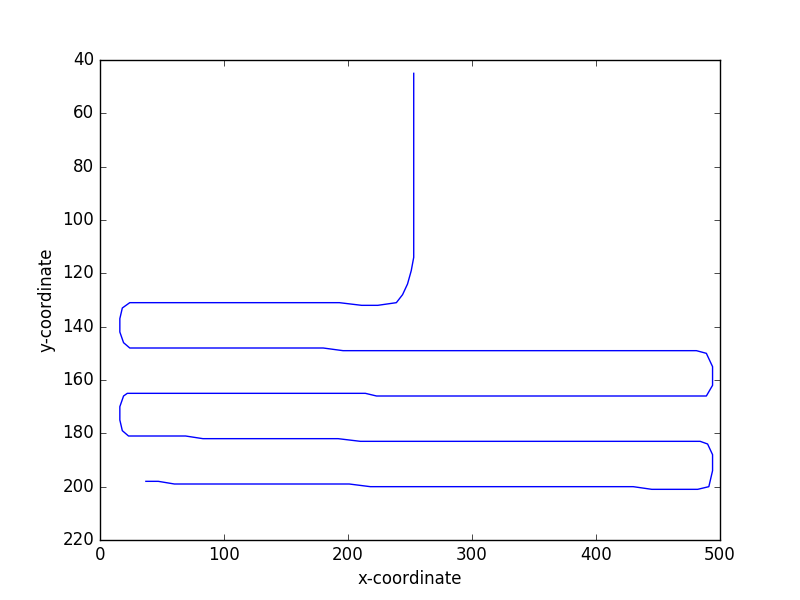
\includegraphics[width=.9\linewidth]{distance.png}
\caption{The points used to compute the distances.}
\end{figure}
\begin{figure}[htb]
\centering
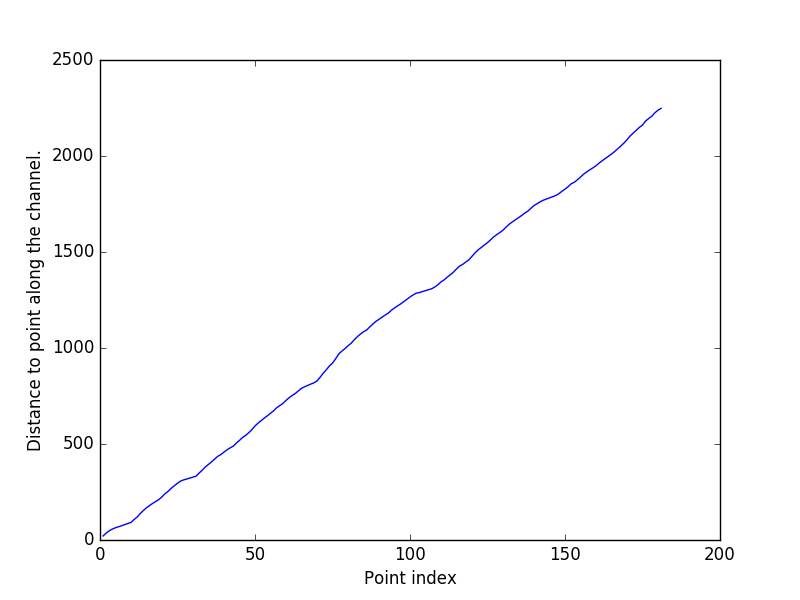
\includegraphics[width=.9\linewidth]{cumulative-distance.png}
\caption{The points used to compute the distances.}
\end{figure}



\section{Frame data}
\label{sec:orgheadline2}

This is data that comes from image analysis. There are 4 columns:
\begin{enumerate}
\item The index of the bubble
\item The area of the bubble in pixels
\item The x-coordinate of the center of mass of the bubble.
\item The y-coordinate of the center of mass of the bubble.
\end{enumerate}

We plot the COMs and the channel distance data here.

\begin{minted}[frame=lines,fontsize=\scriptsize,linenos]{ipython}
import numpy as np
import matplotlib.pyplot as plt
import pycse.orgmode as org
data = np.loadtxt('frame-14.txt', skiprows=1)

indices, areas, x_com, y_com = data.T
plt.figure()
plt.scatter(x_com, y_com, s=areas)
plt.gca().invert_yaxis()
plt.xlabel('x-coordinate')
plt.ylabel('y-coordinate')
plt.plot(x, y, 'b.')
plt.xlim([0, 500])
org.figure(plt.savefig('bubble-x-y.png'), caption='Location of the bubble centers of mass.')

microns2pixels = 2000/85.259
hydraulic_diameter = 121.0  # microns
AREA = 15270  # What is this

# the areas in um^2
areas_um2 = areas * (microns2pixels ** 2)
length_noends = (areas_um2 - np.pi * hydraulic_diameter ** 2 / 4) / hydraulic_diameter

# um^3
volumes = length_noends * AREA + np.pi * hydraulic_diameter ** 3 / 6
\end{minted}

\begin{figure}[htb]
\centering
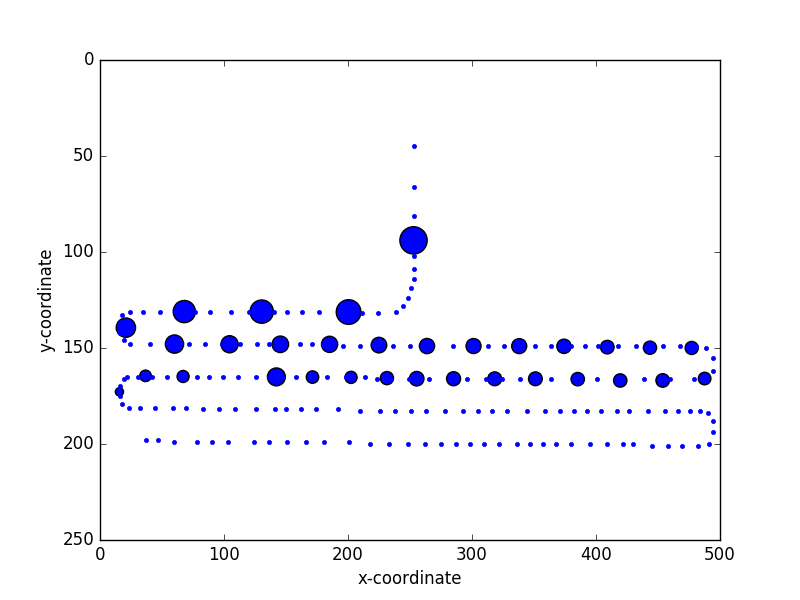
\includegraphics[width=.9\linewidth]{bubble-x-y.png}
\caption{Location of the bubble centers of mass.}
\end{figure}

\section{Calculating the distance to each bubble COM}
\label{sec:orgheadline3}

The principle idea is to consider the data that defines the distance along the channel as a list of segments. We want to find the segment that a particular COM is closest to, and where the intersection is between the points. Then, we just sum the distances up to the point closest to the y-junction, and then add the distance to the COM.

We have points in two lists: x, y for the distances along the channel. We need to create a new list of segments. This list will have one less element in it than the list of points. 

\begin{minted}[frame=lines,fontsize=\scriptsize,linenos]{ipython}
# List of segments, a list of (P1, P2) pairs that define a segment

segments = [[(x[i - 1], y[i - 1]), (x[i], y[i])] for i in range(1, len(x))]
print(len(segments))
print(len(x))
\end{minted}

\begin{verbatim}
181
182
\end{verbatim}


The distance from a point to 
\url{https://en.wikipedia.org/wiki/Distance_from_a_point_to_a_line#Line_defined_by_two_points}

First, we define a function that returns the distance from a point P0 to a segment defined by two points P1 and P2. The points P1 and P2 will be from the channel distance set.
\begin{minted}[frame=lines,fontsize=\scriptsize,linenos]{ipython}
def distance_to_segment(P1, P2, P0):
    """Return distance of P0 to the segement defined by P1 and P2.

    https://en.wikipedia.org/wiki/Distance_from_a_point_to_a_line#Line_defined_by_two_points
    """
    x1, y1 = P1
    x2, y2 = P2
    x0, y0 = P0

    # vertical case
    if x1 == x2:
        #print('vertical segment')
        a = 1.0 
        b = 0.0
        c = -x0
        d = np.abs(a * x0 + c) / np.abs(a)
        x = x1
        y = y0
    # horizontal case
    elif y1 == y2:
        #print('horizontal segment')
        a = 0.0
        b = -1.0
        c = y1
        d = np.abs(b * y0 + c) / np.abs(b)
        x = x0
        y = y1
    # The general case
    else:
        a = (y2 - y1) / (x2 - x1)
        b = -1.0
        c = y2 - a * x2
        d = np.abs(a * x0 + b * y0 + c) / np.sqrt(a ** 2 + b ** 2)
    
        # point of intersection
        x = (b * (b * x0 - a * y0) - a * c) / np.sqrt(a ** 2 + b ** 2)
        y = (a * (-b * x0 + a * y0) - b * c) / np.sqrt(a ** 2 + b ** 2)

    # determine if (x, y) is between P1 and P2
    segment_length = np.sqrt((x1 - x2) ** 2 + (y1 - y2) ** 2)

    # distance of intersection to segment points
    d1 = np.sqrt((x1 - x) ** 2 + (y1 - y) ** 2)
    d2 = np.sqrt((x2 - x) ** 2 + (y2 - y) ** 2)

    # if d1 + d2 == segment length, the intersection is between the segments.
    # We use a tolerance for the comparison. The tolerance is one pixel.
    if np.abs(d1 + d2 - segment_length) < 1:
        return d
    else:
        # return a large number since the intersection is not between the points.
        return 1e10
\end{minted}

Now we get the index to the shortest distance from each point to the segments, and plot them. This will make sure we 

\begin{minted}[frame=lines,fontsize=\scriptsize,linenos]{ipython}
inds = [np.argmin([distance_to_segment(seg[0], seg[1],
                                       com) for seg in segments])
        for com in zip(xs, ys)]


plt.figure()
plt.gca().invert_yaxis()
plt.plot(xs, ys, 'bo')
plt.plot(x, y, 'b.')

# now lines connecting them.

channel_dists = []
for i, ind in enumerate(inds):
    P1, P2 = segments[ind]
    #print(P1, xs[i], ys[i])
    d1 = np.sum(distances[0: ind])
    d2 = np.sqrt((xs[i] - P1[0]) ** 2 + (ys[i] - P1[1]) ** 2)
    channel_dists += [d1 + d2]
    plt.plot([xs[i], P1[0]], [ys[i], P1[1]], 'r-')

org.figure(plt.savefig('closest-dots.png'))

print(len(channel_dists))
\end{minted}

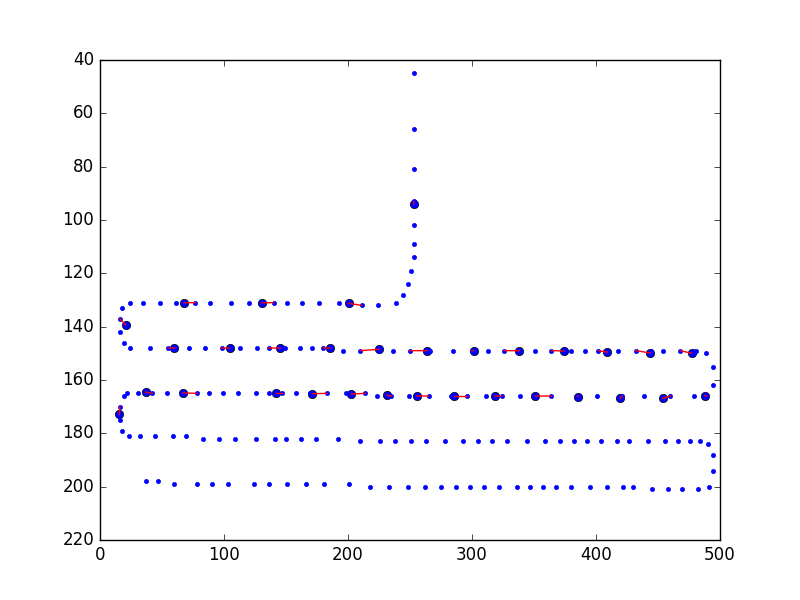
\includegraphics[width=.9\linewidth]{closest-dots.png}
32

Finally, we can plot the areas vs the distance.

\begin{minted}[frame=lines,fontsize=\scriptsize,linenos]{ipython}
plt.figure()
plt.plot(channel_dists, areas, 'bo')
plt.xlabel('Distance (pixels)')
plt.ylabel('Area (pixel$^2$)')
org.figure(plt.savefig('area-vs-dist.png'))
\end{minted}

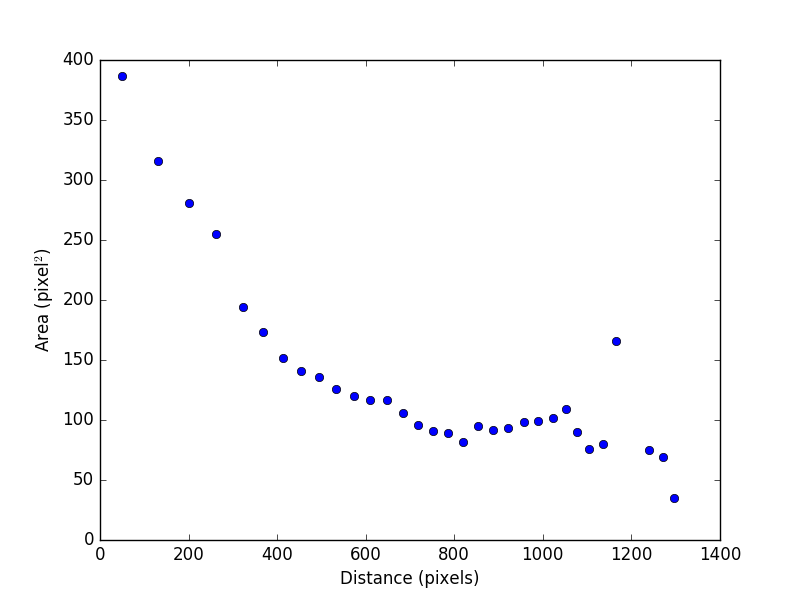
\includegraphics[width=.9\linewidth]{area-vs-dist.png}

It looks like there is one outlier, point 20.

\begin{minted}[frame=lines,fontsize=\scriptsize,linenos]{ipython}
data = [(i, *tup) for i, tup in enumerate(zip(channel_dists, areas, xs, ys))]

org.table([['i', 'distance', 'area', 'x', 'y'], None] + data)
\end{minted}

\begin{center}
\begin{tabular}{rrrrr}
i & distance & area & x & y\\
\hline
0 & 48.9602671503 & 387.0 & 252.847 & 93.948\\
1 & 322.995857341 & 194.0 & 20.875 & 139.401\\
2 & 262.794010213 & 255.0 & 67.971 & 131.025\\
3 & 200.340116802 & 281.0 & 130.425 & 131.052\\
4 & 130.287574005 & 316.0 & 200.475 & 131.269\\
5 & 369.019013956 & 173.0 & 60.072 & 147.957\\
6 & 413.454047525 & 152.0 & 104.507 & 148.053\\
7 & 454.376122061 & 141.0 & 145.429 & 148.074\\
8 & 494.09163654 & 136.0 & 185.144 & 148.091\\
9 & 533.937713054 & 126.0 & 224.951 & 148.491\\
10 & 572.68705739 & 120.0 & 263.709 & 148.987\\
11 & 610.230227332 & 117.0 & 301.252 & 148.979\\
12 & 647.047054582 & 117.0 & 338.069 & 149.009\\
13 & 683.15767843 & 106.0 & 374.179 & 149.113\\
14 & 718.098861293 & 96.0 & 409.1 & 149.544\\
15 & 752.532697781 & 91.0 & 443.524 & 149.841\\
16 & 786.211883204 & 89.0 & 477.182 & 149.977\\
17 & 819.925503504 & 82.0 & 487.592 & 165.908\\
18 & 1270.89043209 & 69.0 & 36.703 & 164.5\\
19 & 1240.55708053 & 75.0 & 67.014 & 164.838\\
20 & 1165.33213826 & 166.0 & 142.238 & 165.049\\
21 & 1136.20278988 & 80.0 & 171.368 & 165.145\\
22 & 1105.14349498 & 76.0 & 202.43 & 165.289\\
23 & 1076.1402768 & 90.0 & 231.389 & 165.673\\
24 & 1052.12050623 & 109.0 & 255.394 & 165.99\\
25 & 1022.36750102 & 102.0 & 285.147 & 166.0\\
26 & 989.218585262 & 99.0 & 318.296 & 166.031\\
27 & 956.392543305 & 98.0 & 351.122 & 166.033\\
28 & 922.280092299 & 93.0 & 385.267 & 166.221\\
29 & 888.243889933 & 92.0 & 419.535 & 166.919\\
30 & 853.795031256 & 95.0 & 453.784 & 166.898\\
31 & 1296.56533113 & 35.0 & 15.671 & 172.814\\
\end{tabular}
\end{center}

This is for sure wrong.
\begin{minted}[frame=lines,fontsize=\scriptsize,linenos]{ipython}
print(xs[4], ys[4], areas[4])

print(np.argmin([distance_to_segment(seg[0], seg[1], [xs[4], ys[4]]) for seg in segments]))
print(segments[44])
\end{minted}

\begin{verbatim}
200.475 131.269 316.0
12
[(196.0, 149.0), (210.0, 149.0)]
\end{verbatim}
\end{document}